% Created 2015-05-09 Sat 23:59
\documentclass[11pt]{article}
\usepackage[utf8]{inputenc}
\usepackage[T1]{fontenc}
\usepackage{fixltx2e}
\usepackage{graphicx}
\usepackage{longtable}
\usepackage{float}
\usepackage{wrapfig}
\usepackage{rotating}
\usepackage[normalem]{ulem}
\usepackage{amsmath}
\usepackage{textcomp}
\usepackage{marvosym}
\usepackage{wasysym}
\usepackage{amssymb}
\usepackage{hyperref}
\tolerance=1000
\usepackage[utf8]{inputenc}
\usepackage[usenames,dvipsnames]{color}
\usepackage{commath}
\usepackage{tikz}
\usetikzlibrary{shapes,backgrounds}
\usepackage{marginnote}
\usepackage{listings}
\usepackage{color}
\usepackage{enumerate}
\hypersetup{urlcolor=blue}
\hypersetup{colorlinks,urlcolor=blue}
\setlength{\parskip}{16pt plus 2pt minus 2pt}
\definecolor{codebg}{rgb}{0.96,0.99,0.8}
\definecolor{codestr}{rgb}{0.46,0.09,0.2}
\DeclareMathOperator{\Dom}{Dom}
\author{Oleg Sivokon}
\date{\textit{<2015-04-03 Fri>}}
\title{Assignment 14, Infinitesimal Calculus}
\hypersetup{
  pdfkeywords={Infinitesimal Calculus, Assignment, Limits of functions},
  pdfsubject={Fourth asssignment in the course Infinitesimal Calculus},
  pdfcreator={Emacs 25.0.50.1 (Org mode 8.2.2)}}
\begin{document}

\maketitle
\tableofcontents


\lstset{language=Lisp,label=fname,numbers=none}
\begin{lstlisting}
(format "\"%s/%s\"" (file-name-directory (buffer-file-name)) f)
\end{lstlisting}

\definecolor{codebg}{rgb}{0.96,0.99,0.8}
\lstnewenvironment{maxima}{%
  \lstset{backgroundcolor=\color{codebg},
    aboveskip=20pt,
    showstringspaces=false,
    frame=single,
    framerule=0pt,
    basicstyle=\ttfamily\scriptsize,
    columns=fixed}}{}
}
\makeatletter
\newcommand{\verbatimfont}[1]{\renewcommand{\verbatim@font}{\ttfamily#1}}
\makeatother
\verbatimfont{\small}%
\clearpage

\section{Problems}
\label{sec-1}

\subsection{Problem 1}
\label{sec-1-1}
\begin{enumerate}
\item Find the domain of $f$ defined as $f(x) = \sqrt{\tan x - 1}$.
\item Find all values of $x$ in segment $[0, \pi]$, for which $\abs{\tan x} \leq \sin 2x}$.
\end{enumerate}

\subsubsection{Answer 1}
\label{sec-1-1-1}
$\tan x > 1$ where $\frac{\pi}{4} < x \bmod \frac{\pi}{2} < \frac{\pi}{2}$.
Since we assume that $f$ is real-valued, we cannot extract roots from negative numbers.

Hence $\Dom(f) = \{x \in \mathbb{R} \; | \; \frac{\pi}{4} < x \bmod \frac{\pi}{2}
    < \frac{\pi}{2}\}$.

\begin{maxima}
programmode: false;
print (plot2d (tan(x),
    [x, -2 * %pi, 2 * %pi], [y, -3, 3],
    [gnuplot_pdf_term_command, 
     "set term cairolatex standalone pdf size 16cm,10.5cm"],
    [gnuplot_postamble,
     "set arrow from pi/4,-3 to pi/4,3 nohead
      set arrow from pi*5/4,-3 to pi*5/4,3 nohead
      set arrow from -2*pi,1 to 2*pi,1 nohead"],
    [ytics, 1, 1, 1], [xtics, 0, 1, 0],
    [label, ["${\\displaystyle \\frac{\\pi}{4}}$", 1.4, 2.4],
            ["${\\displaystyle \\frac{5\\pi}{4}}$", 3.2, 2.4]],
    [title, "Tangent curve"], [pdf_file, %out]));
\end{maxima}

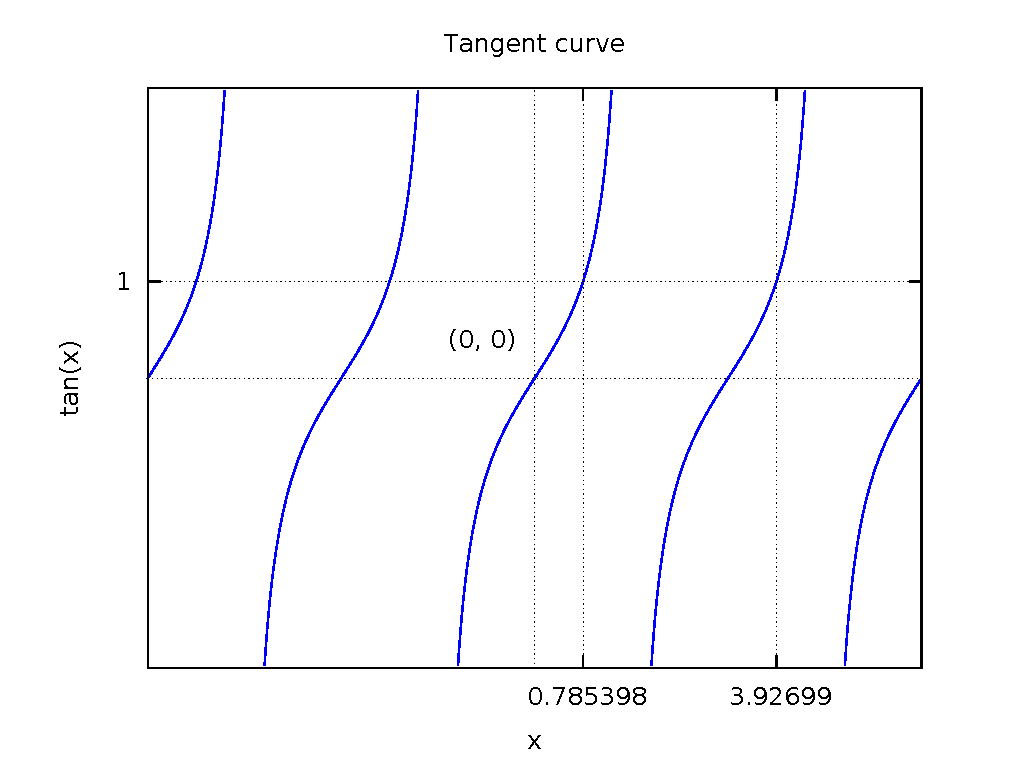
\includegraphics[width=0.9\textwidth]{/home/wvxvw/Documents/uni/infinitesimal-calculus/tangent_x.pdf}
\subsubsection{Answer 2}
\label{sec-1-1-2}
Both functions attain the same values at 0 and $\frac{\pi}{4}$.  But sine is
a concave function and tanget is a convex function, thus tangent must be less
than sine at this interval.  Tangent keeps increasing until $\frac{\pi}{2}$,
while sine will be decreasing until $\frac{3\pi}{2}$, thus, on this interval
tangent is greater than sine.  The functions meet again at $x=\pi$.

\begin{maxima}
programmode: false;
gnuplot_pdf_command: %command;
print(plot2d ([abs(tan(x)), sin(2 * x)],
    [x, -2 * %pi, 2 * %pi], [y, -1.5, 3],
    [gnuplot_pdf_term_command, 
     "set term cairolatex standalone pdf size 16cm,10.5cm"],
    [gnuplot_postamble,
     "set arrow from pi/4,-1.5 to pi/4,3 nohead
      set arrow from pi,-1.5 to pi,3 nohead
      set arrow from -2*pi,1 to 2*pi,1 nohead
      set key spacing 1.8 left bottom"],
    [xtics, 0, 1, 0], [ytics, 1, 1, 1],
    [label, ["${\\displaystyle \\frac{\\pi}{4}}$", 1.4, 2.1],
            ["${\\displaystyle \\pi}$", 3.4, 2.1]],
    [title, "Tangent curve intersecting with sine curve"],
    [pdf_file, %out]));
\end{maxima}

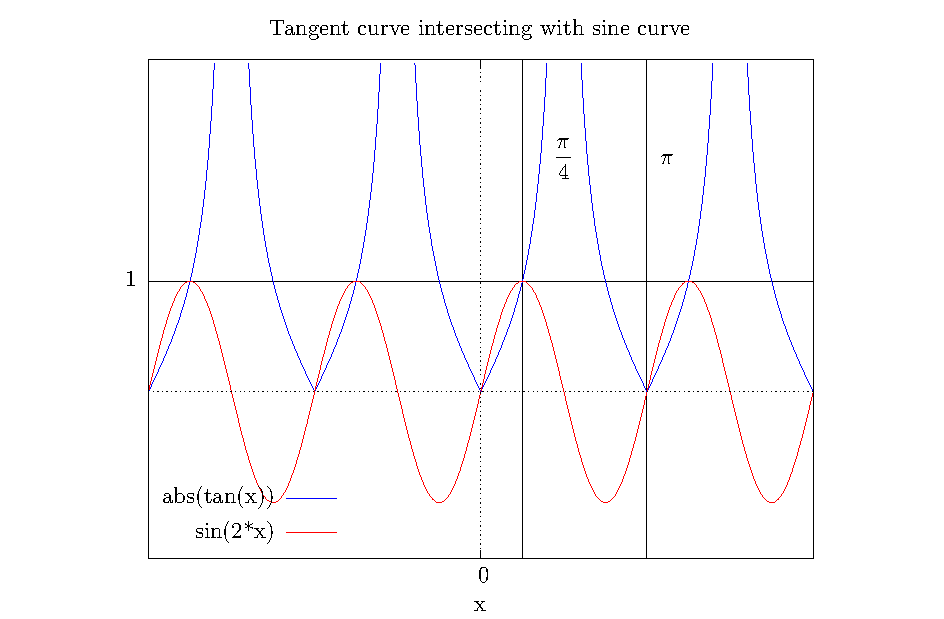
\includegraphics[width=0.9\textwidth]{/home/wvxvw/Documents/uni/infinitesimal-calculus/abstangent_x.pdf}
\subsection{Problem 2}
\label{sec-1-2}
Let $f$, $g$ and $h$ be functions from $\mathbb{R}$ to $\mathbb{R}$.
\begin{enumerate}
\item If $f \circ g = f \circ h$, does it follow $g = h$?
\item If $f \circ g = f \circ h$, and $f$ is one-to-one, does it follow $g = h$?
\item If $f \circ g = f \circ h$, and $f$ is onto, does it follow $g = h$?
\item If $f \circ g$ is increasing, and $f$ is decreasing, does it follow that
      $g$ is increasing?
\item If $f \circ g$ is increasing, and $f$ is one-to-one, does it follow that
      $g$ is monotonic?
\end{enumerate}

\subsubsection{Answer 3}
\label{sec-1-2-1}
No, $g$ and $h$ are not necessarily equal.  Whenever co-domain of $f$
doesn't contain some real number, $g$ and $h$ may differ in that input.
For example, let $f(x) = 2x$, $g(x) = (x \bmod 2) + x$ and
$h(x) = (x \bmod 2) * 2 + x$.  Because $f$ in this example will only
generate even numbers, the $(x \bmod 2)$ term will always be zero,
thus $f \circ g = f \circ h$, but, obviously, $g \neq h$.
\subsubsection{Answer 4}
\label{sec-1-2-2}
No, it isn't sufficient for $f$ to be one-to-one to ensure right-cancellation
property under composition.  The example given in \ref{sec-1-2-1} is applicable
in this case too since whenever $f(x) = f(y)$ so is $x = y$ (since multiplication
does have the cancellation property).
\subsubsection{Answer 5}
\label{sec-1-2-3}
Yes, if $f$ is onto, then the composition is right-cancellable.  Suppose,
for contradiction it wasn't, then for some $y$ $g(y) \neq h(y)$, but
$y = f(x)$ (since by definition of a total function, every element in
its co-domain has an element in its domain).  Hence $g(f(x)) \neq h(f(x))$,
but we are given that $g \circ f = h \circ f$, which is a contradiction.
Hence functions are equal.
\subsubsection{Answer 6}
\label{sec-1-2-4}
No, $g$ doesn't need to be increasing.  Put $g(x) = f(x) = -x$, both $f$
and $g$ are decreasing but $f \circ g = Id$, which is an increasing function.
\subsubsection{Anser 7}
\label{sec-1-2-5}
No, $g$ is not necessarily monotonic.  Put $f(x) = x(-1)^x$ and $g(x) = \abs{x}$.
Then $(f \circ g)(x) = \abs{x(-1)^x} = x\abs{(-1)^x} = x$.  $f \circ g$ is
increasing, $f$ is one-to-one, but $g$ isn't monotonic: it decreases whenever
$x$ is negative and increases whenever $x$ is positive.
% Emacs 25.0.50.1 (Org mode 8.2.2)
\end{document}